% *********************************************************************
% © 2010–2022 Jeremy Sylvestre
%
% Permission is granted to copy, distribute and/or modify this document
% under the terms of the GNU Free Documentation License, Version 1.3 or
% any later version published by the Free Software Foundation; with no
% Invariant Sections, no Front-Cover Texts, and no Back-Cover Texts. A
% copy of the license is included in the appendix entitled “GNU Free
% Documentation License” that appears in the output document of this
% PreTeXt source code. All trademarks™ are the registered® marks of
% their respective owners.
%
% *********************************************************************

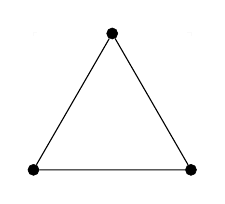
\begin{tikzpicture}[
	vertex/.style={ circle, draw, very thin, fill, inner sep=0pt, minimum size=4pt },
	vertexg/.style={ black!40!white, circle, draw, very thin, fill, inner sep=0pt, minimum size=4pt },
	vertexo/.style={ circle, draw, very thin, inner sep=0pt, minimum size=4pt }
]

\draw[very thin,black!2!white]
  (0.05,0) to (0,0) to (0,0.05)
  (1.95,0) to (2,0) to (2,0.05)
  (1.95,1.75) to (2,1.75) to (2,1.7)
  (0.05,1.75) to (0,1.75) to (0,1.7)
  ;

\begin{scope}
	\node[vertex] at (0,0) (k3v1) {};
	\node[vertex] at (2,0) (k3v2) {};
	\node[vertex] at (1,1.732) (k3v3) {};
	\draw (k3v1) to (k3v2) to (k3v3) to (k3v1);
\end{scope}

\end{tikzpicture}
